\documentclass[a4paper,12pt,numbers=noenddot]{scrreprt}
\setlength{\headheight}{61.24997pt} % Definition der KOMA-Textklasse
\usepackage{amsmath}

\usepackage{tikz} % Add this line to include the tikz package
\usepackage{fancyhdr} 
\usepackage{graphicx}
\usepackage{ragged2e} % Add this line to include the ragged2e package
\usepackage{multicol} % Add this line to include the multicol package
\usepackage{amsfonts}


%%%%%%%%%%%%%%%%%%%%%%
% Set up fancy header/footer
\pagestyle{fancy}
\fancyhead[LO,L]{Deshi}
\fancyhead[CO,C]{Ondas, Óptica y Física Moderna - Ejercicios}
\fancyhead[RO,R]{\today}
\fancyfoot[LO,L]{}
\fancyfoot[CO,C]{\thepage}
\fancyfoot[RO,R]{}
\renewcommand{\headrulewidth}{0.4pt}
\renewcommand{\footrulewidth}{0.4pt}
%%%%%%%%%%%%%%%%%%%%%%

\begin{document}

\begin{minipage}{\textwidth}
  \raggedright
  Considere un bloque de 500 g unido a un resorte ligero de constante de fuerza 2800 [N/m] que oscila horizontalmente sin fricción. \ Si la amplitud máxima de movimiento es como se muestra en la figura, determinar:
\end{minipage}

\begin{itemize}
    \item [\textbf{a)}] \text{\large función \(x(t)\) que describe el movimiento (posición)}
    \item [\textbf{b)}] \text{\large energía total del sistema}
    \item [\textbf{c)}] \text{\large velocidad máxima}
    \item [\textbf{d)}] \text{\large velocidad cuando \(x(t) = 10 \, \text{cm}\)}
\end{itemize}

\begin{center}
\begin{figure}
      \centering
      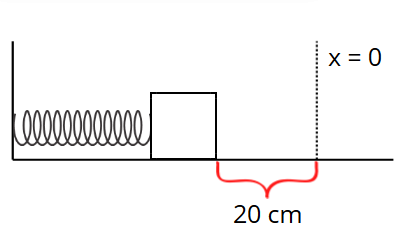
\includegraphics[width=0.5\linewidth]{Ejercicio1.png}
      \caption{bloque con resorte comprimido}
      \label{fig:enter-label}
  \end{figure}
    \end{center}


\begin{figure}[h]\centering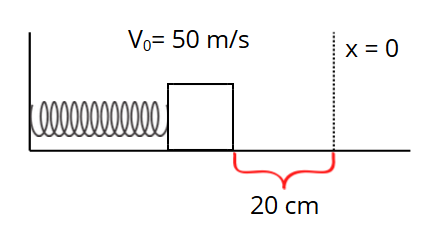
\includegraphics[width=0.5\linewidth]{Ejercicio2.png}\caption{bloque con resorte comprimido y velocidad inicial}\label{fig:enter-label}\end{figure}
    
\end{document}